% 
% ======================================================================
\RequirePackage{docswitch}
% \flag is set by the user, through the makefile:
%    make note
%    make apj
% etc.
\setjournal{\flag}

\documentclass[\docopts]{\docclass}

% You could also define the document class directly
%\documentclass[]{emulateapj}

% Custom commands from LSST DESC, see texmf/styles/lsstdesc_macros.sty
\usepackage{lsstdesc_macros}
\usepackage[utf8]{inputenc}
\usepackage{graphicx}
\usepackage{subfigure}
\graphicspath{{./}{./figures/}}
\bibliographystyle{apj}

% Add your own macros here:


% 
% ======================================================================

\begin{document}

\title{ Impact of the calibration on the performances of the LSST SN survey }

\maketitlepre

\begin{abstract}
We study the impact of the calibration uncertainties, parametrized both as random errors in the zeropoint of each filter ($\delta_{zp}$'s) and as shifts in wavelength of each filter ($\delta_\lambda$'s), on the accuracy of the cosmological constraints that will be extracted from LSST SN survey.
We perform a set of simulations of a typical LSST SNe Ia survey.
The standardization of the SNe Ia, their spectrophotometric evolution, the cosmology and the calibration parameters are fitted at the same time to capture all possible interactions between the parameters.
We show that, when all parameters are left free, a nearly complete degeneracy remains between zero points and cosmology, which can only be lifted by accurate external constraints on the flux scale. We show that an accuracy of the zeropoint determination better than $1\mathrm{mmag}$ is required to extract most of the statistical information LSST supernova sample. In the same way we show that an accuracy of the filter mean positions better than 1$\mathrm{\AA}$ is required.
\end{abstract}

% Keywords are ignored in the LSST DESC Note style:
\dockeys{photometry: calibration}

\maketitlepost

% ----------------------------------------------------------------------
% 

\section{Introduction}
\label{sec:intro}

Our current knowledge of the dark energy is constrained by SN Ia surveys and their analysis. The most recent and best constraints come from the analysis of the SN light curves from the Pantheon Sample (\cite{1710.00845}).
It gives the most precise measurement of dark energy to date with $w = -1.031 \pm 0.040$ in a $w\mathrm{CDM}$ model and $w_0 = -1.011 \pm 0.087$ and $w_a = -0.215 \pm 0.402$ for the $w_0w_a\mathrm{CDM}$ model.

While these uncertainties are dominated by statistics, uncertainty on the photometric color calibration of the SNe Ia, currently of the order of 5 $\mathrm{mmag}$ over 7000$\mathrm{\AA}$, remains one important source of systematic errors.

With LSST, the statistics will increase by a factor between 10 and 30, putting again stringent constraints on calibration accuracy.

In this context the goal of this work is to study the impact of the calibration uncertainties on the performances of a LSST-like survey.
We simulate a typical LSST SNe Ia dataset using the lightweight simulation framework \code{SnSim} (DESC note in prep.) with a light curve generation based on the \code{SALT2} model (\cite{SALT2}).
Then we perform a Fisher analysis with a model including the Supernova standardization parameters, its spectrophotometric evolution, the cosmological and the calibration parameters at the same time, allowing us to compute the covariance matrix of all these parameters.
The performances are evaluated by computing the Figure of Merit ($FoM$) as a function of a priori knowledge on the calibration parameters.

In section \ref{sec::simulated_dataset} we describe the dataset simulation we use in this forecast.
We present our analysis model for the simulated dataset and the way we perform a Fisher analysis to compute the $FoM$ with given calibration uncertainties in §\ref{sec::analysis_model}.
We present our results concerning the performances of the survey for different calibration strategies in section §\ref{sec::results}.
In §\ref{sec::discussion} we discuss the results and we conclude concerning the calibration minimal specifications in §\ref{sec::conclusions}.

% ----------------------------------------------------------------------

\section{Simulated dataset}
\label{sec::simulated_dataset}

\subsection{Cadence}
\label{subsec::cadence}

We assume that the LSST SN survey will be split into two layers:
\begin{itemize}
\item A Wide Fast Deep (WFD) component that will be composed of short exposures ($T_\text{exp} = 2 \times 15\mathrm{s}$) over a large fraction of the sky using a rolling cadence as currently studied within DESC and LSST Project ( SNWG \& Cadence Task Force).
  This survey will allow to discover a large number of nearby SNe Ia ($z < 0.4$).
\item A Deep Drilling Field (DDF) component in which a smaller number of fields will be observed with longer visits ($T_\text{exp} \sim \mathrm{600s}$) to provide distant SNe Ia ($ 0.1 < z < 1$).
\end{itemize}

Observations of a same field in a same filter will be performed with a given period (cadence).
The cadence that will be implemented for the WFD component and the DDF component of the survey is still in discussion.
The goal of this work is to evaluate the impact of calibration systematics on the cosmological measurements, performed with SNe and not to study the impact of the effective cadence and observing conditions.
For this reason we have adopted two nominated scenarii, taken from the current proposed cadences (see Tables \ref{tab:nominal_scenario_wide} \& \ref{tab:nominal_scenario_DDF}).
We also have deliberately simplified the light-curve generation by defining an average cadence in each filter.
This average cadence corresponds to what is delivered by the \code{Altsched} \& \code{Altsched-rolling} nominal requirements for well sampled light-curves. We expect a total of 2000 spectroscopically confirmed SNe Ia per year in the WFD component and 1500 in the DDF.

\begin{table*}[t]
\begin{center}
  \caption{Nominal scenarii for the WFD component that allows to build
    a SN sample complete up to $z \sim 0.4$. The two cadences given in
    each column are for the rolling/standard cadences.}
\label{tab:nominal_scenario_wide}
\begin{tabular}{l|cccc}
\hline
\hline
              & $g$ & $r$ & $i$ & $z$ \\
\hline 
$T_{exp}$      & 30       &   30    &  30        & 30  \\
$m_{5\sigma}$ (limitting mag per visit)  &  24.83   &  24.35   &  23.88    &  23.30  \\
cadence [days]       & 7.7 / 13.6 & 2.9 / 5.6 & 4.3 / 8.2 & 3.3 / 6.7  \\
%Target amplitude SNR & $>30$ & $>40$ & $>30$ & $>20$ \\
\hline
\end{tabular}
\end{center}
\end{table*}

\begin{table*}[t]
\begin{center}
  \caption{A nominal scenario for the DDF component that allows to
    build a SN sample complete up to $z \sim 0.75$.}
\label{tab:nominal_scenario_DDF}
\begin{tabular}{l|cccc}
\hline
\hline
              & $r$ & $i$ & $z$ & $y$ \\
\hline 
$T_{exp}$      & 600 & 600 & 720 & 600 \\
$m_{5\sigma}$ (limitting mag per visit)  & 26.05 & 25.56 & 25.06 & 24.08 \\
cadence  [days]     &  \multicolumn{4}{c}{5 days} \\
%Target amplitude SNR & $>25$ & $>60$ & $>35$ & $>20$ \\
\hline
\end{tabular}
\end{center}
\end{table*}

We build our forecast upon those two nominal scenarii, assuming respectively $30\mathrm{s}$ and $1800\mathrm{s}$ exporures in 4 bands with a regular cadence of 3 days and without loss due to weather. Exact numbers are given in Table \ref{tab:nominal_scenario_wide}  and \ref{tab:nominal_scenario_DDF}. This study will be updated as work on the rolling cadence progresses.

\subsection{Instrument Model and Observing conditions}

We use the most recent model from \cite{SMTN-002} (SMTN-002). The previous model, described in \cite{LSE-40} (LSE-40) has been revised and the new troughput is 40\% lower  in SMTN-002.
We use median observing conditions (same for all epoch) for each filter in Figure \ref{fig:zp}.

\begin{figure}[t]
\begin{center}
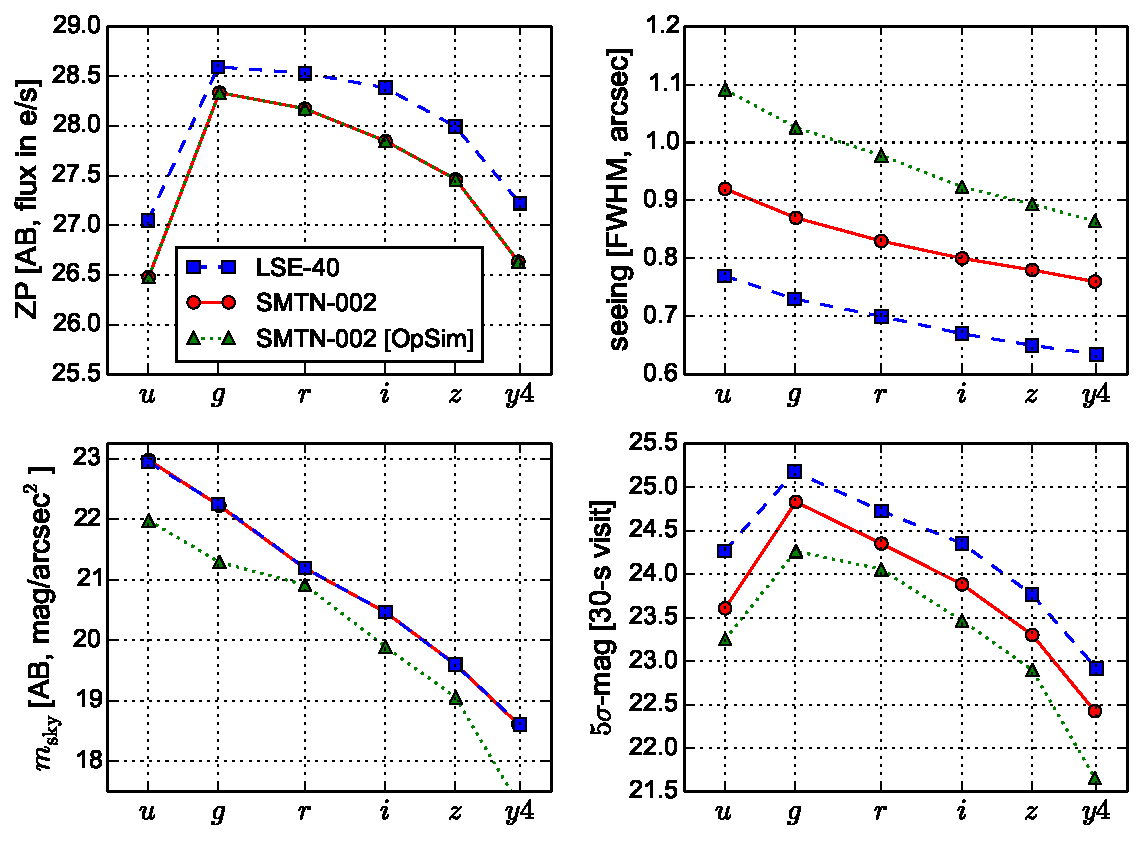
\includegraphics[width=\linewidth]{lsst_model_summary.pdf}
\caption{Parameters of the survey simulation : from left to right and top to bottom we have : zero-points, median seeing, brightness of the background sky (dark time) and survey limiting magnitudes, this Figure is reproduced from \cite{SN-CADENCE} in each $grizy$ band.}
\label{fig:zp}
\end{center}
\end{figure}

\subsection{Simulated SNe}
\label{ssec::snsim}
We use \code{SnSim} (DESC note in prep.) to produce the observed SNe Ia and their light curves with the cadence and observing conditions detailed in the previous sections.
Our study is performed for 1, 5 and 10 years of the LSST SN-survey.
The distribution in redshift of the simulated SNe Ia is shown in Figure \ref{fig:z_distrib}.
Our datasets are redshift limited at $z=0.4$ for the WFD component and $z=0.8$ for the DDF component to ensure their completeness.

\begin{figure}[ht]
  \centering
  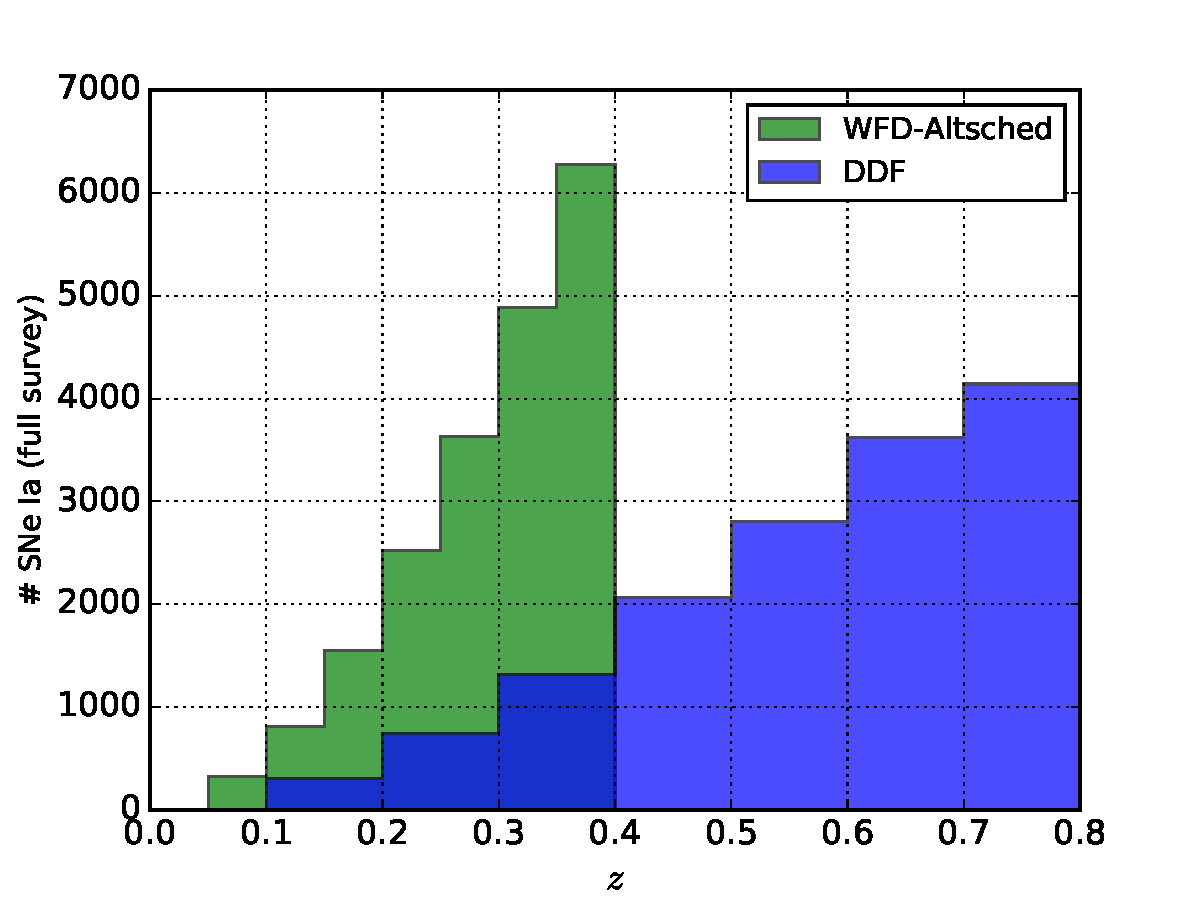
\includegraphics[width=\linewidth]{redshift_distribution_10_seasons.pdf}
  \caption{Redshift distribution of the SNe Ia simulated for the full survey in the WFD (green) and the DDF (blue) components for a total of $35000$ SNe Ia.}
  \label{fig:z_distrib}
\end{figure}
In Figure \ref{fig:lc_examples} we show that in two extreme cases of SNe Ia, one from the WFD component at $z=0.15$ and one from the DDF component at $z=0.71$, the light curves we obtain are well sampled in time with always a measurement at less than 2 days from max luminosity and more than 10 measurements in each band for the light curves (except in $g$ band).
The uncertainty associated to each flux measurement is also reasonably low compared to the light curve amplitude.

\begin{figure*}[t]
\begin{center}
\subfigure[$z = 0.15$]{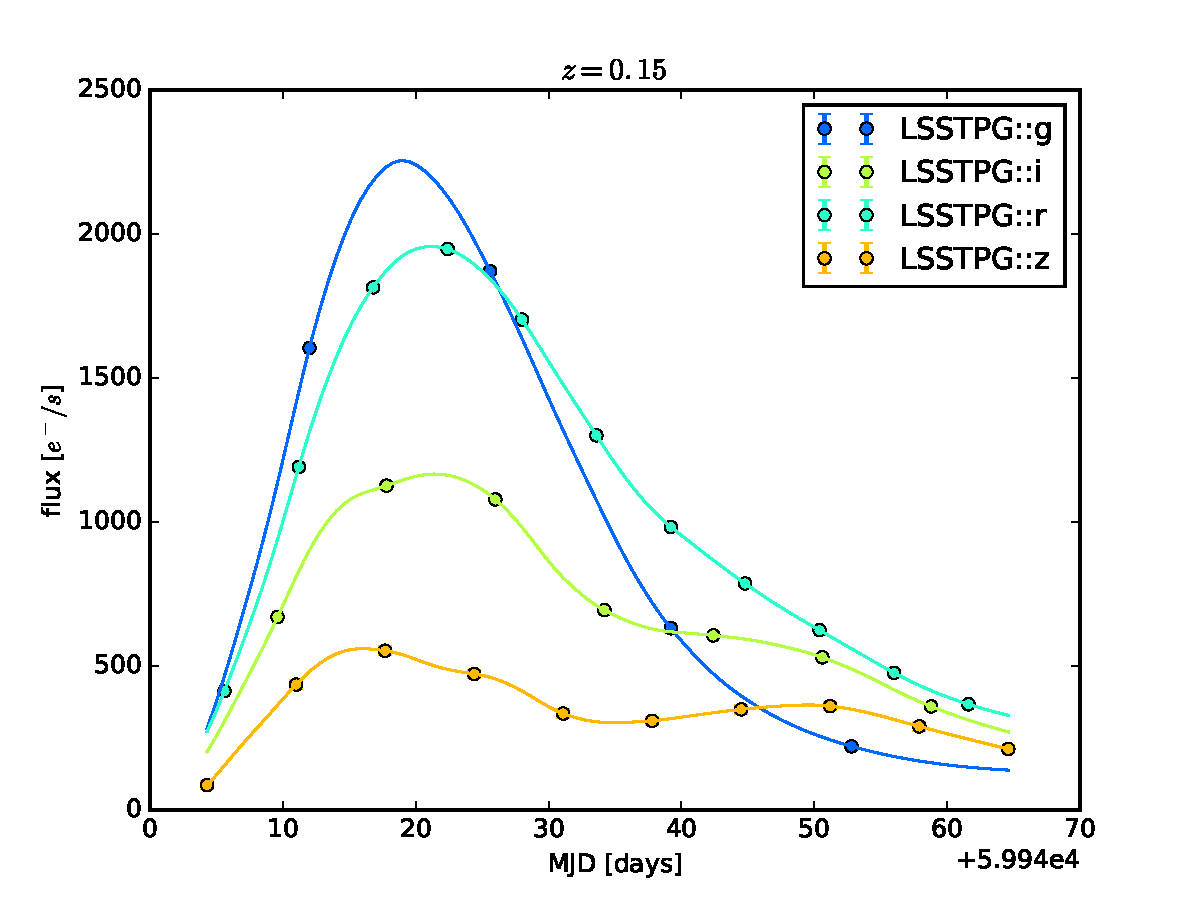
\includegraphics[width=0.48\linewidth]{sn-lc_wide-AltSched_z015.pdf}}
\subfigure[$z = 0.71$]{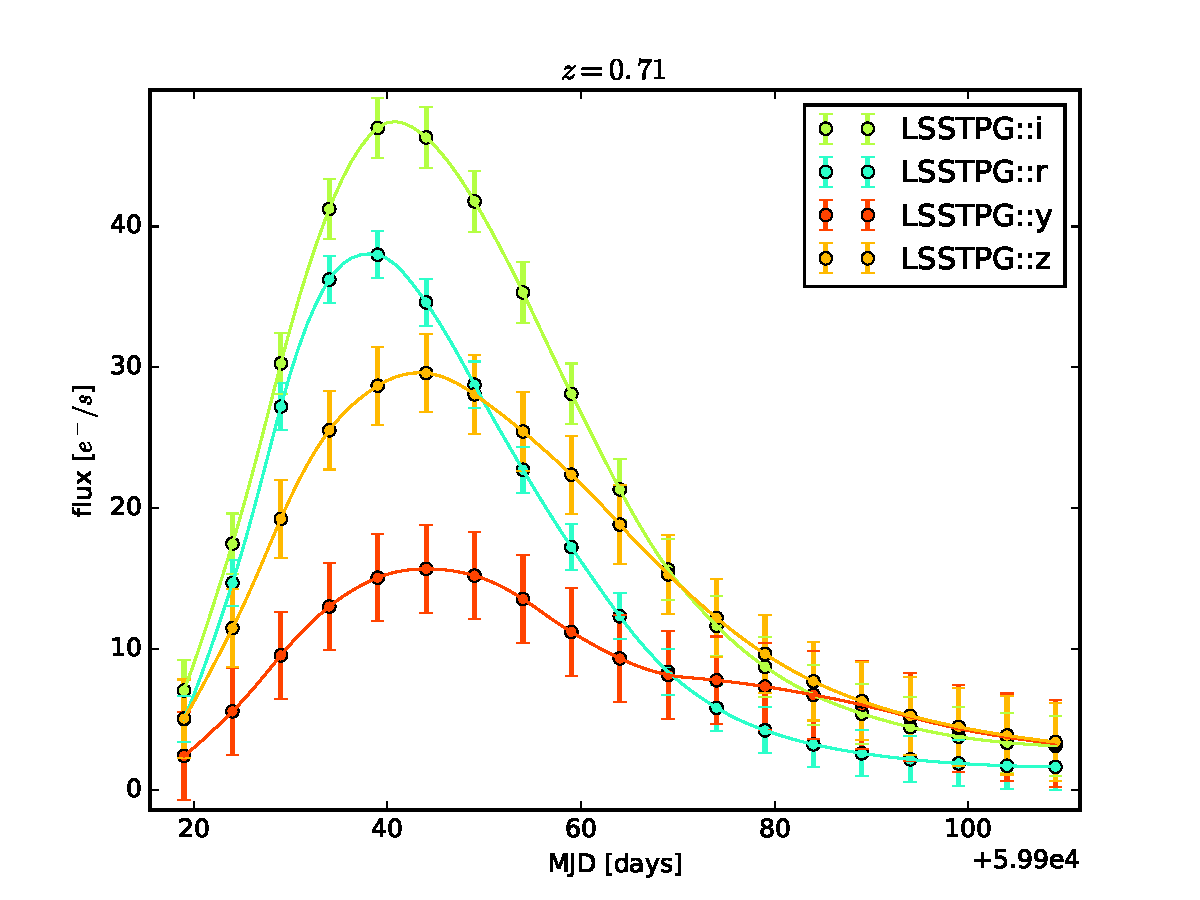
\includegraphics[width=0.48\linewidth]{sn-lc_deep_z071.pdf}}\\
\caption{Light curves for a SN Ia measured in the WFD component at $z=0.15$ in $griz$ bands (left) and a SN Ia measured in the DDF component at $z=0.71$ in $rizy$ bands (right).}
\label{fig:lc_examples}
\end{center}
\end{figure*}

Finally, we show in Figure \ref{fig:sigmas} that in each layer the \code{SALT2} color $c$ uncertainty is always below 30$\mathrm{mmag}$ in both components and for all SNe Ia in the considered redshift range.
Also time of maximum luminosity $t_0$ uncertainty is below 0.5 days and the stretch of the simulated SN Ia $x_1$ uncertainty is below 0.5, which are the threshold of \cite{1401.4064} for SNe Ia to be included in the training sample.

\begin{figure*}[t]
\begin{center}
\subfigure[wide]{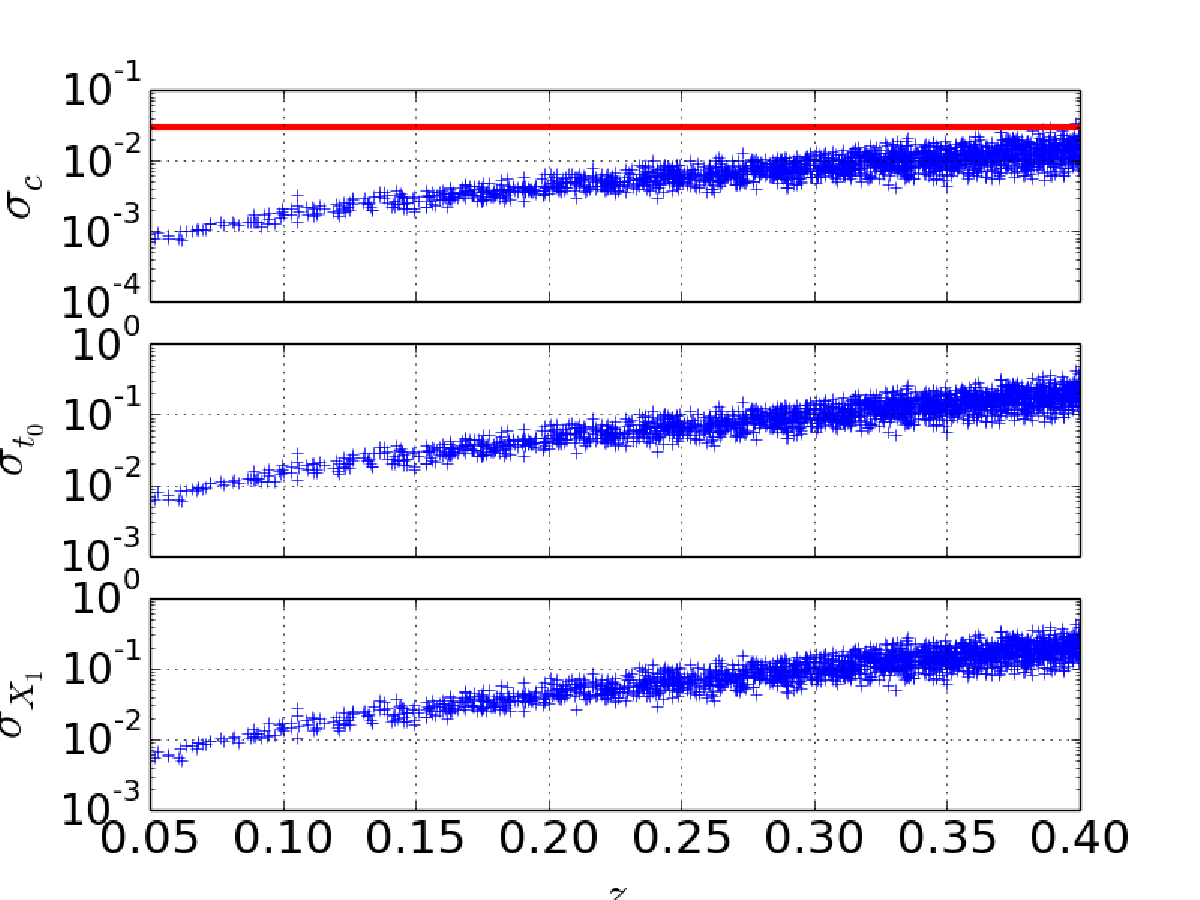
\includegraphics[width=0.48\linewidth]{lsst_wide_WFC_sigmas_2000SNe.pdf}}
\subfigure[deep]{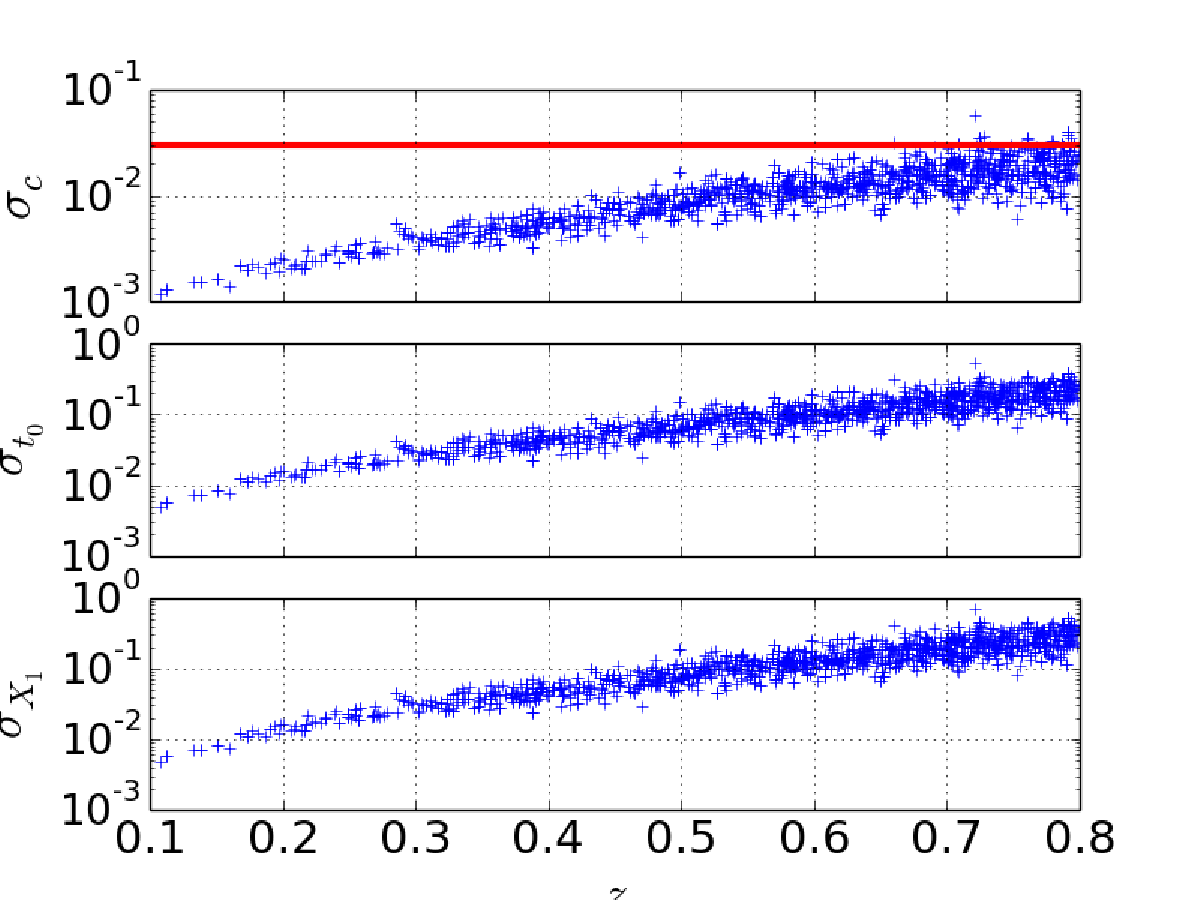
\includegraphics[width=0.48\linewidth]{lsst_deep_DDF_sigmas_1500SNe.pdf}}\\
\caption{Uncertainty of the color, the time of maximum luminosity and the stretch of each SN Ia (from top to bottom) in the wide (left) and the deep (right) layers. The horizontal red line corresponds to $\sigma_c = 0.03$ which is the threshold on the accuracy on the color of a well measured SN Ia}
\label{fig:sigmas}
\end{center}
\end{figure*}

% ----------------------------------------------------------------------

\section{Analysis Model}
\label{sec::analysis_model}

We now describe how we evaluate the analysis of the SNe Ia data as it is likely to be performed in 2020+.
We have developed a pipeline that implements : (1) Light curves fit, (2) training of a spectrophotometric model, (3) standardization of the SNe Ia and (4) a cosmology.

\subsection{Model details}
\label{subsec::model_details}
We want our model to be representative of a real analysis, while avoiding the complexity and numerical clumsiness of a complete spectroscopic model.
In order to avoid the need of including spectra in our simulation, we will mimick their effect on broadband quantities.
Calibration uncertainties induce redshift dependent errors on magnitude and color as SNe at different redshifts are observed in different bands.
It is thus of primary importance to account for the fact that the SN spectrophotometric model will be trained on the data, and not considered as known.
On the contrary, the SN light-curve shape (stretch) is expected to be well constrained thanks to the good sampling (\ref{ssec::snsim}), and calibration uncertainties do not strongly impact shapes (e.g. \cite{1401.4064} Figure 6).
We thus can simplify our model by neglecting the time evolution of the SNe Ia, only modeling the flux of each measured SN Ia in each used band considered, interpolated at the day of maximum luminosity in the restframe $B$ band (hereafter $t_0$).
The flux of a given SN Ia measured at $t_0$ in a band $b$ (in $\mathrm{e^{-}/s/cm^2}$) can be modeled as follows:

\begin{equation}
\label{eq::flux_model}
\varphi_b = \frac{1}{1+z} \times \frac{10^{-10}}{d_L^2(z, \theta_\text{c})}\times \int \frac{10^{-10}\lambda}{hc} S\left(\frac{\lambda}{1+z}\right) T_b(\lambda) d\lambda \text{ ,}
\end{equation}
where $z$ and $d_L$ are respectively the redshift and the luminosity distance (in $\mathrm{Mpc}$) of the given supernova,
$\theta_\text{c}$ is the vector of the cosmological parameters (depending on the model we choose to use),
$S\left(\frac{\lambda}{1+z}\right)$ is the SED of a standard SN Ia (in $\mathrm{erg/s/\AA/cm^2}$) at 10 $\mathrm{pc}$ and $T_b(\lambda)$ is the transmission of the detector in a band $b$ (in $\mathrm{e^-/phot}$).
Translating equation \ref{eq::flux_model} into magnitudes:
\begin{equation}
\begin{split}
\label{eq::raw_model}
m_b = &\mu(z, \theta_\text{c}) + 25 + 2.5\log_{10}(1+z) \\
&- 2.5\log_{10}\int \frac{10^{-10}\lambda}{hc} S\left(\frac{\lambda}{1+z}\right) T_b(\lambda) d\lambda \text{ ,}
\end{split}
\end{equation}
where $\mu(z, \theta_\text{c})$ is the SN distance modulus ($\mu(z, \theta_\text{c}) = 5\log_{10}(d_L)$).

We assume SN spectrum to be smooth enough to perform a Taylor expansion at the first order around a given wavelength $\bar\lambda_b$ over the wavelength range of each observer-frame filter, so that:
\begin{equation}
\int \lambda S\left(\frac{\lambda}{1+z}\right) T_b(\lambda) d\lambda \approx \int \left( \bar{S}\left(\frac{\bar\lambda_b }{1+z}\right) + (\lambda - \bar\lambda_b)\frac{\partial\bar{S}}{\partial\lambda}\left(\frac{\bar\lambda_b }{1+z}\right)\right)\times \lambda T_b(\lambda) d\lambda \text{ .}
\end{equation}

By choosing $\bar\lambda_b$ as $\bar\lambda_b = \frac{\int \lambda^2 T_b(\lambda) d\lambda}{\int \lambda T_b(\lambda) d\lambda}$, we set the integration of the first order term to 0, so that we have:

\begin{equation}
\int \lambda S\left(\frac{\lambda}{1+z}\right) T_b(\lambda) d\lambda \approx \bar{S}(\frac{\bar\lambda_b }{1+z}) \times \int \lambda T_b(\lambda) d\lambda \text{ .}
\end{equation}

We note that it will be possible to modelize the restframe SN spectrum because we are observing a large number of SNe Ia at multiple redshifts, each in four restframe bands.

% We perform a polynomial expansion around the central wavelength of the passband $\bar\lambda_b$.
% Since we work only with photometric data, we perform a linear approximation of the spectrum over a range centered on the mean wavelength of the passband $\bar\lambda_b$.
% We have then:

% \begin{equation}
% \int \lambda S\left(\frac{\lambda}{1+z}\right) T_b(\lambda) d\lambda \approx \bar{S}(\frac{\bar\lambda_b }{1+z}) \times \int \lambda T_b(\lambda) d\lambda
% \end{equation}
% where $\bar{S}(\frac{\bar\lambda_b }{1+z})$ is the mean of the spectrum over the considered passband.
% $\bar\lambda_b$ evaluated as $\bar\lambda_b = \frac{\int \lambda^2 T_b(\lambda) d\lambda}{\int \lambda T_b(\lambda) d\lambda}$ for the term of $1^{st}$ order to vanish in the integral.

Eq. \ref{eq::raw_model} becomes:          
\begin{equation}
  m_b = \mu(z, \theta_\text{c}) + 25 + 2.5\log_{10}(1+z) - 2.5 \log_{10} \bar{S}(\bar\lambda_b ) + \mathcal{Z}_b \text{ ,}
\end{equation}
where $\mathcal{Z}_b = -2.5 \log \int \frac{10^{-10}\lambda}{hc} T_b(\lambda) d\lambda$ is the band zeropoint.

As we will show later, care must be taken while modeling the SED of the supernovae and its characterization shall remain free to evolve with the input data.
We emulate a \code{SALT2} parametrization and write:
\begin{equation}
-2.5\log_{10}S(\bar\lambda_b) = M_X + P(\frac{\bar\lambda_b}{1+z}) + cQ(\frac{\bar\lambda_b}{1+z}) + c\beta \text{ ,}
\end{equation}
where $P(\frac{\bar\lambda_b}{1+z})$ plays the role of the mean restframe spectrum of a "standard" SN Ia, $M_X$ is a normalization factor accounting for the restframe absolute luminosity of each SN, $Q(\frac{\bar\lambda_b}{1+z})$ is a color law accounting for the color variation of each SN around the mean SN spectrum and $\beta$ is the brighter-bluer parameter that relates flux variation to SNe color.
We also introduce here the \code{SALT2}-like color $c$ of each SN.
We decompose the mean spectrum over a B-spline basis of degree 2, and the color law over a polynomial of fourth degree.

$\beta$ plays the role of the degree 0 in $Q( \lambda )$. We fix it in $Q( \lambda )$ by imposing $Q(\lambda_B) = 0$ and $Q(\lambda_V) = -1$, $\lambda_B$ and $\lambda_V$ being respectively Johnson's $B$ and $V$ band mean wavelengths.
We also fix $P(\frac{\bar\lambda_b}{1+z})$ normalization and its color to cut degeneracies with respectively $M_X$ and $Q(\frac{\bar\lambda_b}{1+z})$.

Incorporated to the model it gives:

\begin{equation}
\begin{split}
\label{eq::model}
m_b = &M_X + 25 + \mu(z, \theta_\text{c}) + 2.5\log_{10}(1+z) \\
&+ P(\frac{\bar\lambda_b }{1+z}) + cQ(\frac{\bar\lambda_b }{1+z}) + c\beta + \mathcal{Z}_b \text{ .}
\end{split}
\end{equation}

At this stage some degeneracies appear between these different parameters.
The way to handle these degeneracies is to add priors to our model.
If $J$ is the matrix of the derivatives  of our model with respect to all free parameters (columns) for all light curve amplitudes measured (lines), we can vertically add matrices to $J$ for each prior, corresponding to one or more "additionnal" measurements:
\begin{equation}
J =
\begin{pmatrix}
  J \\
  J_\text{priors}
\end{pmatrix} 
\end{equation}

In parallel, if $C$ is the covariance matrix of our measurements, we add diagonally the covariance matrix of the prior to $C$:
\begin{equation}
C =
\begin{pmatrix}
  C & 0 \\
  0 & C_\text{priors}
\end{pmatrix} \text{ .} 
\end{equation}

In our case we add the following priors:
\begin{itemize}
\item We fix all the $M_X$'s at a same value to cut degeneracies with the distance moduli but with a dispersion of 10\% to account for the intrinsic dispersion of the SNe Ia absolute maximum luminosity that has been observed in previous SN Ia analyses.
\item Since we use a $w_0w_a$ cosmology, $\theta_\text{c} = \{ \Omega_m$, $\Omega_k$, $w_0$, $w_a$, $H_0$, $\Omega_bh^2 \}$, we add a Planck prior from \cite{1502.01589}, which brings us the information on $H_0$ and $\Omega_k$ we would not get with the SNe Ia only.
\end{itemize}

% ----------------------------------------------------------------------

\subsection{Calibration parameters}
\label{subsec::calib_uncertainties}
The core of this work is about the way we handle the calibration errors and incorporate them in \ref{eq::model}.
We describe them with two different parameter subsets:
\begin{itemize}
\item $\delta zp$'s, that takes into account the error we make on the normalization of the transmission in each band.
There is one associated to each filter we use.
\item $\delta \lambda$'s, which is the error made in observer frame on the mean wavelength position of each filter. 
\end{itemize}

The model (hereafter $\mathcal{M}$) finally becomes :
\begin{equation}
\begin{split}
m_b = & M_X + 25 + \mu(z, \theta_\text{c}) + 2.5\log_{10}(1+z) + \mathcal{Z}_b \\
&+ P(\frac{\bar\lambda_b  + \textcolor{red}{\delta\lambda_b}}{1+z}) + cQ(\frac{\bar\lambda_b  + \textcolor{red}{\delta\lambda_b}}{1+z}) + {c\beta} + \textcolor{red}{\delta zp_b} \text{ .}
\end{split}
\end{equation}

\subsection{Structure of the Calibration covariance matrix}
\label{subsec::covmat}
These calibration parameters are associated to a calibration covariance matrix $C_s$.
The structure of $C_s$ depends on the calibration strategy. In particular it is generally non diagonal because of the interplay between $zp$ and filter positions.
The state of the art concerning SNe Ia flux measurements consists in comparing their flux directly with calibrated astrophysical standards.
We assume that the zeropoint of a band $b$ is obtained using the flux measurement of a calibrated astrophysical standard, which is modeled as:
\begin{equation}
zp_b = \int T_b(\lambda) S_{std}(\lambda) d\lambda + e_{zp_b} \text{ ,}
\end{equation}
where $T$ is the transmission of the instrument, $S_{std}$ is the spectrum of the astrophysical standard and $e_{zp_b}$ is a random noise with $cov(e_{zp_b}) = \sigma_{zp_b}^2$.
This way of measuring flux implies that if we make an error on the wavelength position of the filters, the flux integration of the standard will not be what we expect, which in turn leads to an error on the zeropoint of the band.
\begin{equation}
\begin{split}
zp_b &= \int \bar T_b(\lambda) S_{std}(\lambda) d\lambda + e_{zp_b} + \frac{\partial \int{T_b(\lambda)S(\lambda)d\lambda}}{\partial \bar\lambda_b }\delta\bar{\lambda}_b\\
&= \bar{zp}_b + e_{zp_b} + \frac{\partial zp_b}{\partial \bar\lambda_b }\delta\bar\lambda_b 
\end{split}
\end{equation}
We then have:
\begin{equation}
\begin{pmatrix}
  zp \\
  \bar\lambda_b 
\end{pmatrix}
=
\begin{pmatrix}
  1 & \frac{\partial zp}{\partial \lambda} \\
  0 & 1
\end{pmatrix}
\begin{pmatrix}
  e_{zp_b} \\
  \delta\bar\lambda_b 
\end{pmatrix}
+
\begin{pmatrix}
  \widehat{zp} \\
  \widehat{\bar{\lambda_b}}
\end{pmatrix}
\end{equation}
We define $\frac{\partial zp}{\partial \lambda}$ as the change in zeropoint for $1 \mathrm{\AA}$ of filter position error, obtained by comparing the integrated flux of an astrophysical standard (P330E in this case) in a reference filter and in a shifted filter.
We have:
\begin{equation}
C_s = cov
\begin{pmatrix}
  zp \\
  \bar\lambda_b
\end{pmatrix}
=
\begin{pmatrix}
  1 & \frac{\partial zp}{\partial \lambda} \\
  0 & 1
\end{pmatrix}
\begin{pmatrix}
  \sigma_{zp}^2 & 0 \\
  0 & \sigma_{\lambda}^2
\end{pmatrix}
\begin{pmatrix}
  1 & 0 \\
  \frac{\partial zp}{\partial \lambda} & 1
\end{pmatrix}\text{ .}
\end{equation}
We put the values in Table \ref{tab::calib_derivatives}, then $C_s$ becomes :
\begin{equation}
\label{eq::cov_calib}
C_s = 
\left( \begin{array}{cc|cc} \sigma^2_{ zp_{g}} + (\sigma_{\lambda_g} \frac{\partial zp_g}{\partial \lambda_g})^2 & 0 & \frac{\partial zp_g}{\partial \lambda_g} \sigma^2_{ \lambda_g} & 0 \\ 0 & \ddots & 0 & \ddots \\ \hline \frac{\partial zp_g}{\partial \lambda_g} \sigma^2_{ \lambda_g} & 0 & \sigma^2_{\lambda_{g}} & 0 \\ 0 & \ddots & 0 & \ddots \end{array} \right) \text{ .}
\end{equation}

\begin{table*}[t]
\begin{center}
\caption{$\delta zp$'s derivatives with $\delta\lambda$'s computed using P330E spectrum.}
\label{tab::calib_derivatives}
\begin{tabular}{l|ccccc}
\hline
\hline
  & $g$ & $r$ & $i$ & $z$ & $y$ \\
\hline 
  $\frac{\partial\delta zp}{\partial\delta \lambda}$ $[\mathrm{mmag/\AA}]$& 0.026 & 0.18 & 0.24 & 0.23 & 0.22\\
\hline
\end{tabular}
\end{center}
\end{table*}

% ----------------------------------------------------------------------

% \subsection{Model degeneracies}
% \label{ssec::model_deg}

% At this current stage our model have some degeneracies that we must get rid of.
% The way to handle this degeneracies is to add priors to our model.
% If $J$ is the matrix of the derivatives  of our model with respect to all free parameters (columns) for all light curve amplitudes measured (lines), we can vertically add matrices to $J$ for each prior, corresponding to one or more "additionnal" measurements:
% \begin{equation}
% J =
% \begin{pmatrix}
%   J \\
%   J_\text{priors}
% \end{pmatrix} 
% \end{equation}

% In parallel, if $C$ is the covariance matrix of our measurements, we add diagonally the covariance matrix of the prior to $C$:
% \begin{equation}
% C =
% \begin{pmatrix}
%   C & 0 \\
%   0 & C_\text{priors}
% \end{pmatrix} 
% \end{equation}

% In our case we add the following priors:
% \begin{itemize}
% \item The spectrum normalization, to cut degeneracy with the distance modulus $\mu$ that could increase while $M_X$ decrease.
% \item The spectrum color, that is degenerated with the color law.
% \item The fact that the color law is fixed at $\lambda_B$ and $\lambda_V$ respectively mean wavelength of the $B$ and $V$-bands
% \item We fix the dispersion of the $M_X$'s at 14\% because otherwise we have degeneracies with the distance moduli.
% \item Since we use a $w_0w_a$ cosmology, $\theta_\text{c} = \{ \Omega_m$, $\Omega_k$, $w_0$, $w_a$, $H_0$, $\Omega_bh^2 \}$, we add a Planck prior, extracted from Planck 2015 results(\cite{1502.01589}), which brings us the information on $H_0$ and $\Omega_k$ we wouldn't get with the SNe Ia only.
% \end{itemize}


% ----------------------------------------------------------------------

\subsection{Error propagation}
\label{sec::linalg}

% The analysis of a real SN Ia data sample would need us to perform a simultaneous fit marginalized over all Table \ref{tab:params} parameters. Because of the high number of parameters, to ensure a quicker execution and avoid memory issues we work with sparse matrices.
The model $\mathcal{M}$ do take into account simultaneously all Table \ref{tab:params} parameters. Because of the high number of parameters, to ensure a quicker execution and avoid memory issues we work with sparse matrices.

\begin{table*}[t]
\begin{center}
\label{tab:params}
\caption{Summary of our model free parameters}
\begin{tabular}{l|ccccccccc}
\hline
\hline
Free parameters & $M_X$ & $\theta_\text{c}$ & $\theta_P$ & $\theta_Q$ & $c$ & $\beta$ & $\mathcal{Z}$ & $\delta zp$ & $\delta \lambda$ \\
\hline
\# parameters & $N$ & 6 & 31 & 5 & $N$ & 1 & 5 & 5 & 5 \\
\hline
\end{tabular}
\end{center}
\end{table*}

The $\chi^2$ associated to the model $\mathcal{M}$ is:
\begin{equation}
\chi^2 = \sum_{sb}\frac{[m_{sb} - \mathcal{M}(s, b, \vec\theta)]^2}{\sigma_{sb}^2} \text{ .}
\end{equation}

In order to easily propagate the errors, we linearize $\mathcal{M}$ around the maximum likelihood, using the SN parameters that have been put into the dataset simulation in order to produce the light curves.

The linearized model $\mathcal{M'}$ describe the data as follows::
\begin{equation}
\mathcal{M'} = J \times \vec\theta
\end{equation}
Where $J$ contains the derivatives of our model with respect to all free parameters (columns) for all light curve amplitude measured (lines) and $\vec\theta$ the vector of all our free parameters (details in Table \ref{tab:params}).

The normal equation for this $\chi^2$ is:
\begin{equation}
J^TC^{-1}J = J^TC^{-1}y
\end{equation}
where $y$ and $C$ are respectively our measurements and their covariance matrix.

Finally we add the calibration covariance matrix $C_s$ (explicited in §\ref{subsec::calib_uncertainties}) as a prior to our model (as in §\ref{subsec::model_details}).
For the moment we have to keep in mind that these value are not fixed, and we are going to make this study for several examples of what would be the calibration accuracy for the LSST SN survey.

Since we want to study the performances of the survey, we do not need to perform a fit.
In order to get the uncertainties of our model parameters, we compute the Fisher information matrix, that we call $H$, around the maximum likelihood.
\begin{equation}
H = J^TWJ
\end{equation}
where $W = C^{-1}$.

According to Cramér–Rao theorem, the inverse of $H$ is a lower bound on the covariance matrix of all our free parameters, including cosmological parameters.
So it allows us to know which constraints a given dataset and a given calibration will put on the cosmological parameters.

To ensure the consistency of our analysis and the way we propagate the calibration uncertainties, we test our pipeline on the JLA data sample: instead of simulating an LSST dataset, we use the real light curve amplitudes and SNR in each of the observed band published in \cite{1401.4064}.
The JLA calibration covariance matrix has a similar design to the one considered here, including the zeropoint calibration errors, the filter position errors antd the correlation terms.
We thus run our analysis pipeline on this dataset, using the calibration covariance matrix (provided by \cite{1401.4064}), and assuming a $\Lambda\mathrm{CDM}$ cosmology.
We obtain an uncertainty on $w$ of 5.2\% (stat+sys) when \cite{1401.4064} obtained 5.7\%.
In JLA, the statistic uncertainty as the systematics are both 4\%. In our case, the statistic uncertainty is undervalued as we are at 3.4\%, but we are only wrong at 0.1\% concerning the statistic uncertainty with 3.9\% in our analysis.
We thus show that the impact of calibration on the performances of a SN survey is well reproduced by our analysis.

% ----------------------------------------------------------------------

\section{Results}
\label{sec::results}
We study the performances of a given survey on the determination of cosmological parameters through the Figure of Merit ($FoM$), defined as:
\begin{equation}
FoM = \frac{1}{\sqrt{det(cov(w_0, w_a))}} \text{ .}
\end{equation}
We then perform a block inversion of $H$.
We modify the calibration strategy by changing the $\sigma_{\delta \lambda}$'s and the $\sigma_{\delta zp}$'s in $C_s$ (eq \ref{eq::cov_calib}) which impact $H$ through $W$.
We compute the $FoM$ with $\sigma_{\delta zp} = \sigma_{zpg} = \sigma_{zpr} = \sigma_{zpi} = \sigma_{zpz} = \sigma_{zpy}$, and $\sigma_{\delta\lambda} = \sigma_{\lambda_g} = \sigma_{\lambda_r} = \sigma_{\lambda_i} = \sigma_{\lambda_z} = \sigma_{\lambda_y}$ at 20 different values from $\sigma_{\delta zp} = 10^{-5}\mathrm{mag}$ to $\sigma_{\delta zp} = 1\mathrm{mag}$ and $\sigma_{\delta \lambda} = 10^{-2}\ \mathrm{\AA}$ to $\sigma_{\delta \lambda} = 100\mathrm{nm}$.
With highly cadenced survey (\code{Altsched-rolling} with respect to \code{Altsched}), we obtain higher SNR, but we do not observe any difference between the two sets of cadence in the WFD component detailed in \ref{subsec::cadence} in terms of performances on the cosmological parameters knowledge.
It shows that below a given cadence, the light curve amplitude SNR is negligible with respect to the intrinsic dispersion of the SN Ia fluxes.
We present these results for one, five and ten years of survey in Figure \ref{fig:fom_grids} for the standard WFD cadence.

We observe three distinct areas: a plateau on the lower left where the
survey performances saturate and are statistic dominated; an inflection
region surrounding this plateau where statistical and systematic errors
have similar weight; and a surounding plateau of low performances where
the systematic errors dominate.
In the statistically dominated regime, the asymptotic $FoM$ reaches 320 for a 5 year survey, and 680 for a 10 years survey.

\begin{figure*}[t]
\begin{center}
\subfigure[1 year]{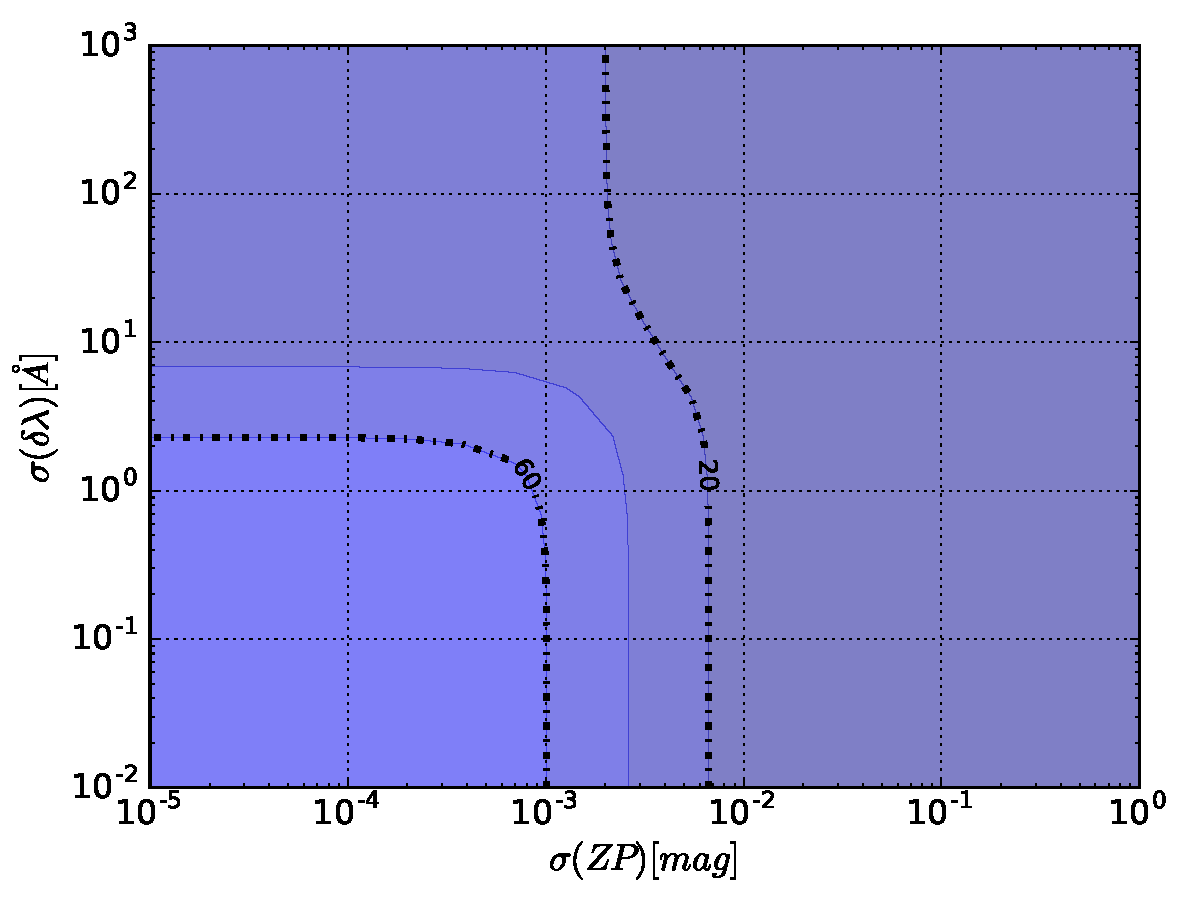
\includegraphics[width=0.48\linewidth]{FoM-grid_1-seasons_AltSched_with-training.pdf}}
\subfigure[5 years]{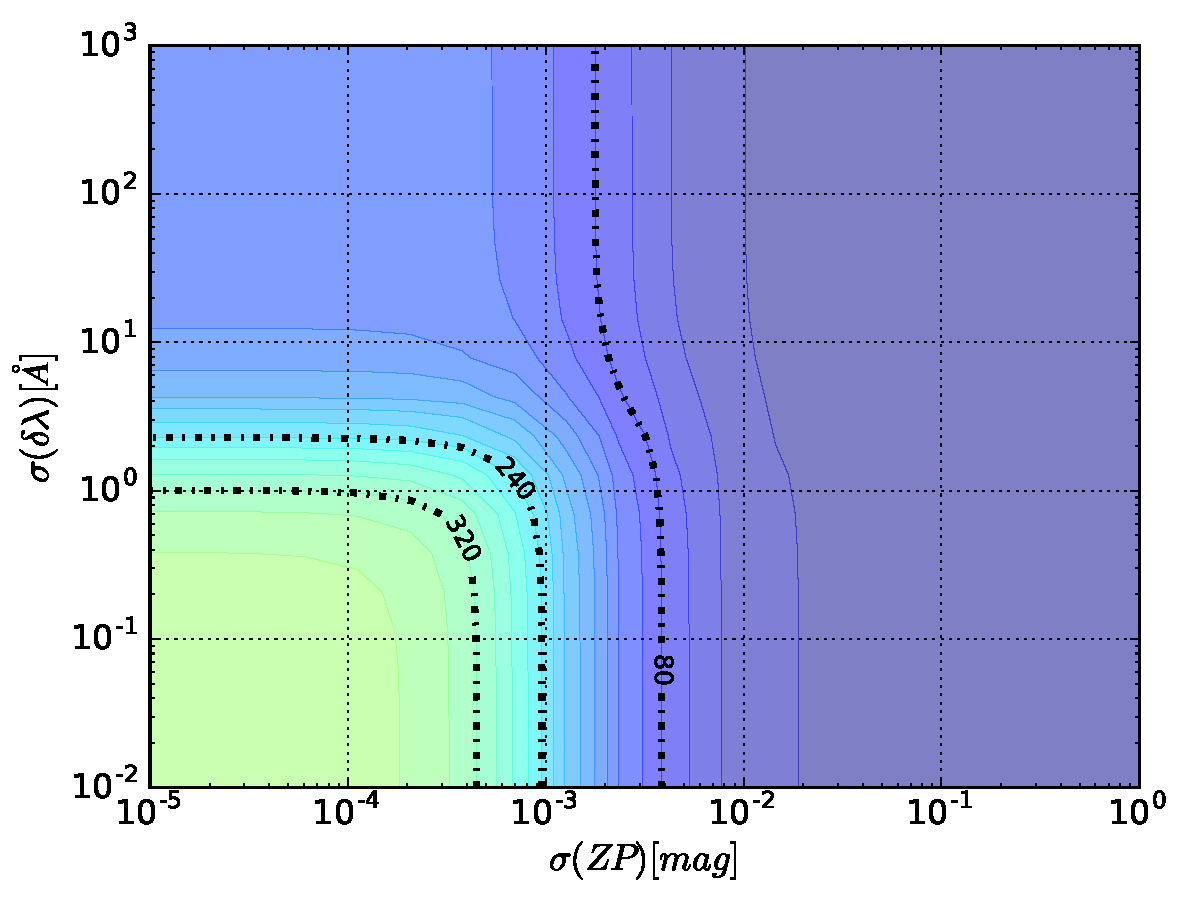
\includegraphics[width=0.48\linewidth]{FoM-grid_5-seasons_AltSched_with-training.pdf}}\\
\subfigure[10 years]{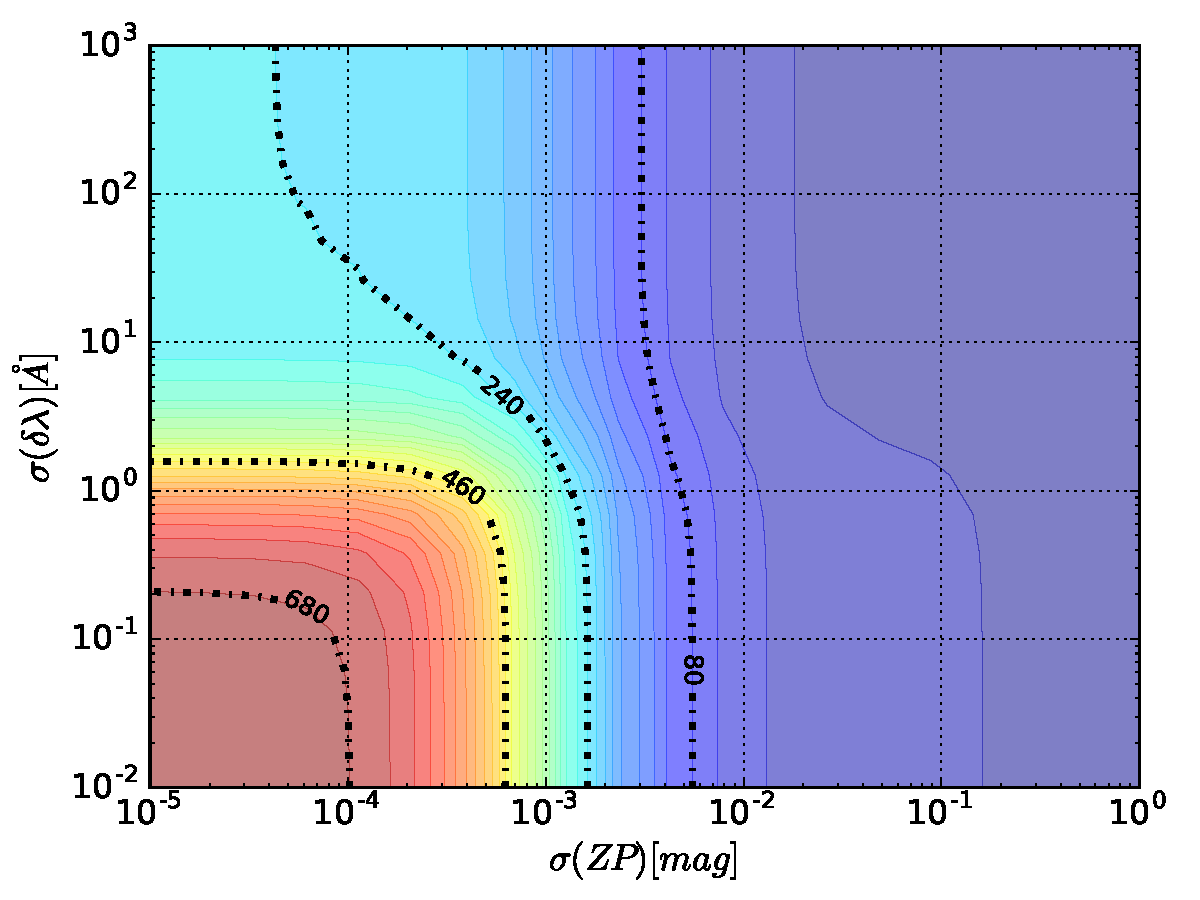
\includegraphics[width=0.48\linewidth]{FoM-grid_10-seasons_AltSched_with-training.pdf}}
\subfigure[10 years (slice)]{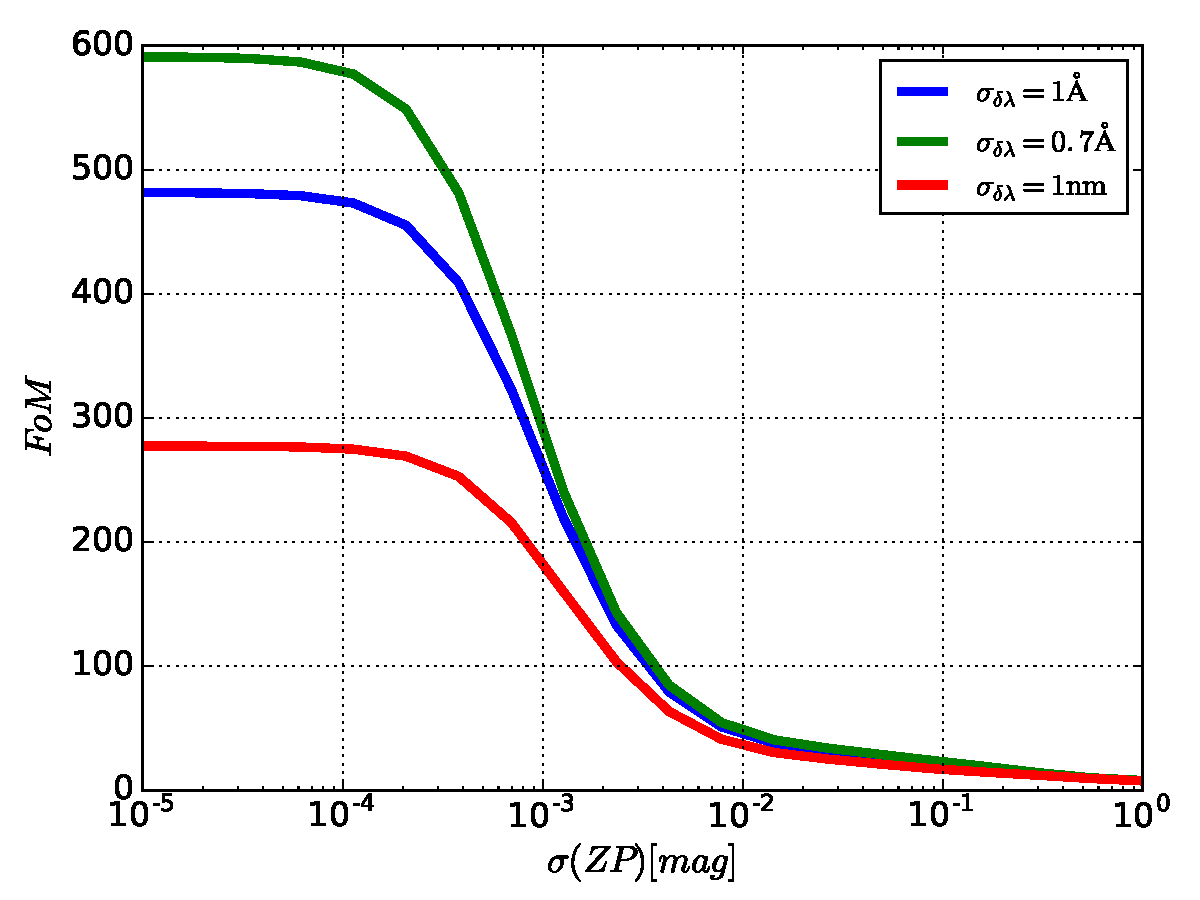
\includegraphics[width=0.48\linewidth]{FoM-plot_10-years.pdf}}
\caption{ (a), (b) \& (c) : $FoM$ that can be achieved at one, five and
  ten years (full SN-survey). The $FoM$ iso-countous are represented on
  a same color base for the 3 plots. Indicative iso-contours are
  represented in dot-dashed lines at some given $FoM$. The x-axis
  represents the a priori uncertainty on the filters zeropoint while
  the y-axis represents the uncertainty on the mean filter
  position. Each small iso-contour is separated from the others by 20
  points in the $FoM$. \\ (d) : Slices of (c) at
  $\sigma_{\delta\lambda} = 1\mathrm{\AA}$ in
  blue, $\sigma_{\delta\lambda} = 0.7\mathrm{\AA}$ in green and
  $\sigma_{\delta\lambda} = 1\mathrm{nm}$ in red.}
\label{fig:fom_grids}
\end{center}
\end{figure*}

\subsection{Zeropoints}
Concerning the photometric calibration, with the current uncertainties on the $\delta zp$'s at $5 \mathrm{mmag}$ (\cite{1401.4064}), we observe that for a 1 year survey we obtain a $FoM$ of $\approx 30$, while improving it to $1 \mathrm{mmag}$ leads to a $FoM$ of 60.
For a 5 years survey, having a photometric calibration between 1 and 2 $\mathrm{mmag}$ appears to be mandatory to extract at least 50\% of the performances the statistics could grant us.
Finally we can see that a calibration below the mmag level should be reached to make use of the full statistics of the LSST SN-survey.

\subsection{Filters}
Concerning the uncertainty on filter mean wavelength position : For a one year survey, we need the filter mean position uncertainty to be at  $\approx 1\mathrm{nm}$ for for it not to be predominant with respect to the statistics.
At 5 years the transition occurs at $2 \mathrm{\AA} < \sigma_{\delta\lambda} < 4 \mathrm{\AA}$.
For a full 10 years survey, we show that if the filter
average wavelength is known to $10 \mathrm{\AA}$, as the LSST Project requirements
state, most of the statistical power of the dataset is lost. In order
for the sytematic and statistical errors to have an equivalent
weight, we need a requirement ten times more stringent, i.e. a knowledge
of the filter mean wavelength of the order of $1 \mathrm{AA}$ or better.
The main difference in behaviour compared to the photometric calibration is that that the $FoM$ seems to reach a non-zero plateau at low accuracy on the filter mean position.
It is due to an auto-calibration phenomenon of the uncertainty on $\delta\lambda$, we come back to this in the next session.

% ----------------------------------------------------------------------

\section{Discussion}
\label{sec::discussion}
\subsection{Impact of the model training}
\label{ssec::training}
As a parallel work, we study the impact of the spectro-photometric supernova model training on the $FoM$ estimate.
By considering the $\theta_P$ parameters of the spectro-photometric model as free, we decouple the supernova model training from the analysis, in particular removing all covariances between the supernova model reconstruction and the color calibration of the survey.
Figure \ref{fig:fom_wout_training} shows that, compared to what we obtain with the training, we are making a large overestimation of the performances of the survey, that goes along with an underestimation of the impact of photometric calibration.
\begin{figure}[ht]
  \centering
  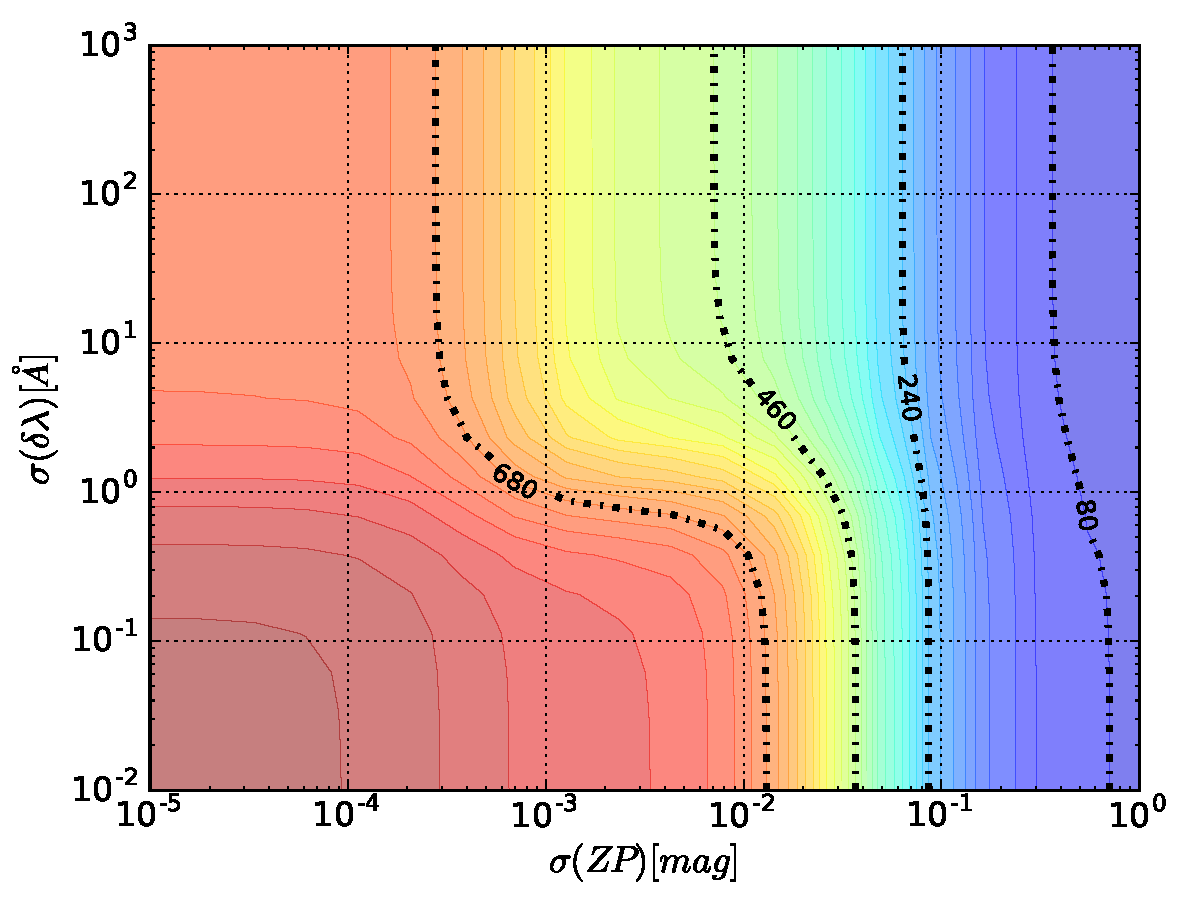
\includegraphics[width=\linewidth]{FoM-grid_10-seasons_AltSched_no-training.pdf}
  \caption{Evolution of the $FoM$ with respect to the filter position
    uncertainty and the filter zeropoint as in Figure
    \ref{fig:fom_grids} but without training the spectrophotometric
    model. As the transition area is around $\sigma_{zp} = 1\mathcal{mmag}$, here it is at $\sigma_{zp} = 100\mathcal{mmag}$.}
  \label{fig:fom_wout_training}
\end{figure}
We also notice that the $FoM$ is different from 0 even when the \textit{a priori} knowledge on the zero-points is minimal.
The higher \textit{a posteriori} knowledge of the zeropoints is an artifact assuming a perfectly calibrated SN model which calibrates our zeropoint.

\subsection{Filter position auto calibration}
In Figure \ref{fig:fom_grids} we observe that the $FoM$ does not fall to 0 at very low filter knowledge.
The filter mean positions are calibrated by the SNe Ia in what we call an auto-calibration.
The \textit{a posteriori} uncertainty the filter mean positions saturates at a value of $\sim 1 \mathcal nm$ while increasing the \textit{a priori} uncertainty at higher values.
This phenomenon is possible because our spectrophotometric model, trained on photometric data only, is slowly variating.
We also assume a perfectly known redshift, while taking into account redshift uncertainty into account could prevent this phenomenon.
In our model hypotheses we also parametrize the filter uncertainties very simply as their mean wavelength positions, a more complexe parametrization could have interesting results on this auto-calibration.

Since we can already spot the area where statistics and systematics are equivalent, this work still give us the main information on the requirements we should reach.
A later version of this work will take into account these cautions.


% As has been said in section \ref{sec::results}, the $FoM$ does not
% fall to zero with a dramatical decrease of the accuracy on the filter
% mean position, this seems to occur because of an auto-calibration
% phenomenon.  We have added the spectral diversity of the type Ia SNe
% as a pedestal on the uncertainty of the flux measured for each SN in
% each band, which weakened the auto-calibration.  Caution should be
% exercised before concluding that such an autocalibration of filter
% passband could occur in the analysis of actual data:
% \begin{itemize}
% \item we assume a perfectly known redshift.
% \item there is no high frequency spectral features in our photometric SN model
% \item We use a simple parametrization of the filter uncertainties
% \end{itemize}
% Since we can already spot the transition area where a small
% improvement in the filter position calibration leads to a great
% improvement of the performances, this work still give us the main
% information on the requirements we should reach. A later version of
% this work will take into account these cautions


% We can notice that, assuming a smooth cosmology, there does not seem to be degeneracies between the filter positions and cosmological parameters.
% This is because filter shifts introduce wiggles in the Hubble Diagram (see Figure \ref{fig:lambda_der}) that can be spotted and erased by the fit.

% ----------------------------------------------------------------------

\section{Conclusion}
\label{sec::conclusions}
In this study, we implement a fast and realistic end to end simulation
of a LSST SN survey.  We take simultaneously into account the
spectrophotometric evolution of the SNe Ia, the cosmology and the
calibration parameters.  We have shown the necessity to take into
account the training of the spectrophotometric model over the dataset
to obtain realistic results from this type of study.  The exposed
relation highlights the necessity to calibrate the throughput of the
LSST filters with a precision better than $10^{-3}$ level in order to
bring LSST statistical power above the systematic error floor. Finaly
we found that the uncertainty on the filters positions seem to have a
lesser effect on the performances.  We explain this phenomenon by the
fact that we are fitting together a smooth cosmology and the SN
spectrophotometric model, and the fact that the size and the quality
of the SN sample we have simulated is very high.  This particular
point will be investigated in a second iteration of this work, in a
first time by adding an uncertainty on the redshift of each SN
allowing for spatial inhomogeneities of filter passbands and in a
second time by adding the phase dimension of the spectrophotometric
evolution of the SNe Ia. We can finally see that we are in a good
agreement with the DESC SRD v0.9 concerning the calibration
requirements.


% ----------------------------------------------------------------------

\subsection*{Acknowledgments}

%Here is where you should add your specific acknowledgments, remembering that some standard thanks will be added via the \code{acknowledgments.tex} and \code{contributions.tex} files.

%% 
This is the text imported from \code{acknowledgments.tex}, and will be replaced by some standard LSST DESC boilerplate at some point.
% 


\input{contributions}

%{\it Facilities:} \facility{LSST}

% Include both collaboration papers and external citations:
\bibliography{lsstdesc,main}

\end{document}
% ======================================================================
% 
